\newpage
\section{Data Exploration}
%\begin{figure}[H]
%  \centering
%  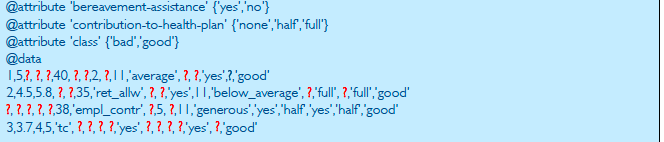
\includegraphics[width=.5\linewidth]{arffmissing}
%\end{figure}
It's the preliminary exploration of the data aimed at \textbf{identifying their most relevant characteristics}. In this step many important information inside the data can be found like outliers, missing values , data ranges etc. which are crucial to pick the right preprocessing  and data mining steps.\\
\subsection{Summary statistics}
Summary statistics are numbers that summarize properties of data : location,mean,spread,skewness ,standard deviation ,mode, percentiles, etc.
\begin{itemize}
\item \textbf{Frequency}\\
Percentage of time value occurs in the data set ( used with categorical data)
\item \textbf{Mode}\\
Most \textbf{frequent} attribute value ( used with categorical data)
\item \textbf{Mean}\\
Most common measure of the location of a set of points. It is \textbf{very sensitive} to outliers.$$ \text{mean(x)} = \bar{x} = \frac{1}{m} \sum \limits_{i=1}^{m}x_i $$
\item \textbf{Median}\\
The median is the value separating the higher half from the lower half of a data sample. \[ \text{median(x)}= 
  \begin{cases}
    x_{r+1} & \quad \text{if } m \text{ is odd , like m=2r+1}\\
    \frac{1}{2}(x_r + x_{(r+1)})  & \quad \text{if } m \text{ is even , like m=2r}
  \end{cases}
\]
\item \textbf{Percentiles}\\
Given an ordinal or continuous attribute x and a number p between 0 and 100  the p-th percentile is a value $x_p$ of x such that $p\%$ of the observed values of x are less than $x_p$
\item \textbf{Trimean}\\
Is the weighted mean of the first , second and third quartile : $$TM= \frac{x_{25}+2x_{50}+x_{75}} {4}$$
\item \textbf{Truncated mean}\\
Discards data \textbf{above} and \textbf{under} a certain percentile.
\item \textbf{Interquartile mean}\\
$$X_{IQM} = \frac{2}{n} \sum \limits_{i=0.25n+1}^{0.75n} x_i$$
\item \textbf{Range}\\
Difference between max and min
\item \textbf{Variance}\\
$$ \text{variance(x)}= s^{2}_x  = \frac{1}{m-1} \sum \limits_{i=1}^{m}(x_i - \bar{x})^2$$. Sensitive to outliers (see below for robuster statistics) 
\item \textbf{Average absolute deviation}\\
$$ AAD(x)  = \frac{1}{m} \sum \limits_{i=1}^{m} |x_i - \bar{x}|$$
\item \textbf{Mean absolute deviation}\\
$$ MAD(x) = \text{median}\left( \{  |x_1-\bar{x}|,...,|x_m - \bar{x}|\} \right)$$
\item \textbf{Interquartile range}\\
$$ \text{interquartile range(x)} = x_{75\%} - x_{25\%} $$
\item \textbf{Correlation analysis}\\
Given two attributes it measures how strongly one attribute implies the other ,based on available data ( \textbf{does not imply causation}).
\begin{itemize}
\item \textbf{Numerical values}\\
Compute the c\textbf{orrelation coefficient}, Pearson's product
\item \textbf{Ordinal variables}\\
Compute \textbf{Spearman} rank correlation coefficient
\item \textbf{Categorical variables}\\
Compute the $\chi ^2$ \textbf{statistic test} which tests the hypothesis that A and B are independent.
\item \textbf{Binary variables}\\
Compute \textbf{point-biserial} correlation
\end{itemize}
\item \textbf{Outliers}\\
They are data objects that do not comply with the general behaviour or model of data,that is , values that appear as \textbf{anomalous}. Most data mining methods consider outliers \textbf{noise} or \textbf{exceptions}. They can be detected using : \begin{itemize}
\item Statistical tests that assume a distribution or probability model for the data
\item Distance measure where objects that are substantial distance from any other cluster are considered outliers
\item Deviation based models identify outliers by examining differences in the main characteristics of the objects in a group
\end{itemize}
They are usually \textbf{filtered out by trimming} or replaced with the \textbf{Winzorsing technique} : a $10\%$ Winsorizing considers $5{th}$ and $95^{th}$ percentiles , setting values below the $5^{th}$ to the $5^{th}$ itself and above the $95^{th}$ to the $95^{th}$ itself.  
\end{itemize}

\subsection{Normalisation}
When attributes have vastly different \textbf{scales}  (e.g. age vs income) it is necessary to normalize them.
\begin{itemize}
\item \textbf{Range normalisation}\\
$$ x'_i= \frac{x_i - min_i x_i}{max_i x_i - min_i x_i}$$
\item \textbf{Standard score normalisation}\\
$$x'i=\frac{x_i - \mu }{\sigma}$$
\end{itemize}

\subsection{Visualisation}
Visualisation is the conversion of data into \textbf{visual} or \textbf{tabular} format so that the characteristics of data and relationships among data points can be analysed ( detected \textbf{patterns,trends,outliers...})\\
\begin{itemize}
\item \textbf{Bar plot}\\
They use horizontal or vertical bars to compare categories. One axis shows the \textbf{compared categories} the other axis represents a \textbf{discrete value}. Variants are \textbf{grouped bar graphs} (clustered in groups of more than one) and \textbf{stacked bar graphs} (bars divided into subparts to show cumulative effect)
\item \textbf{Histograms}\\
They are a graphical representation of \textbf{distribution of data}. They estimate the probability distribution of continuous variables depicting adjacent rectangles whose areas are proportional to the frequency of the observations in the interval. The height of each bar indicates the number of objects
\begin{figure}[H]
 \centering
 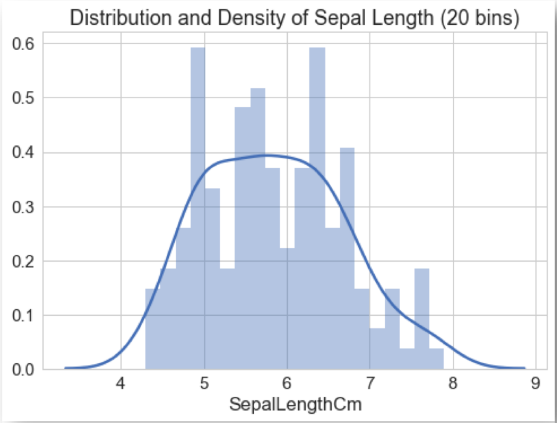
\includegraphics[width=.5\linewidth]{histogram}
\end{figure}
\item \textbf{Scatter plots}\\
Attributes values determine the position inside the scatter plot. Usually scatter plots are two dimensional but also three dimensional scatter plots exist.
\item \textbf{Box plots}\\
They represent another way of representing the distribution of data
\begin{figure}[H]
 \centering
 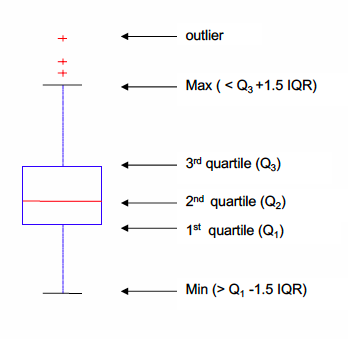
\includegraphics[width=.5\linewidth]{boxplot}
\end{figure}
\end{itemize}

\subsubsection{Multiple dimension at once visualisation}
When dealing with more than 2 dimensions some plots allow to represent the data showing all the dimensions at once:
\begin{itemize}
\item \textbf{Chernoff faces}\\
Associates each attribute with a characteristic of a face. The values of each attribute determine the appearance of the corresponding facial characteristic : each sample becomes a \textbf{separate face}.
\begin{figure}[H]
 \centering
 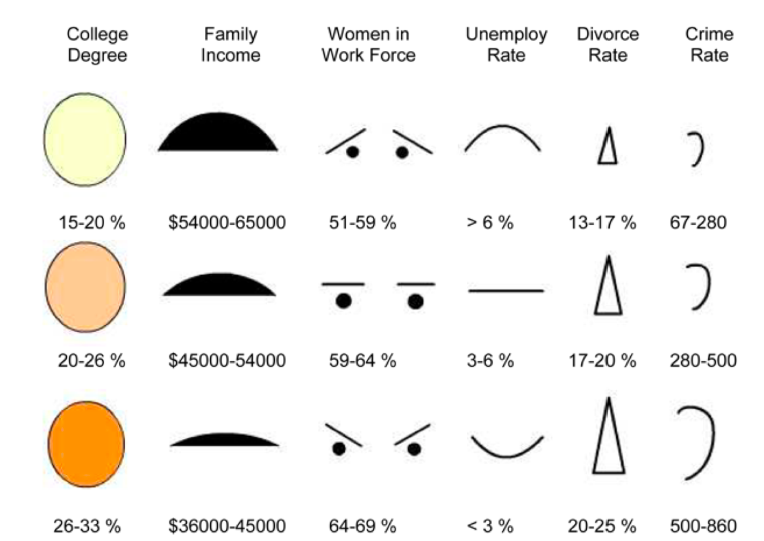
\includegraphics[width=.5\linewidth]{chernoff}
\end{figure}
\item \textbf{Star plots}\\
Similar approach that uses axes radiate from a central point.The line connecting the values of an object is a polygon
\begin{figure}[H]
 \centering
 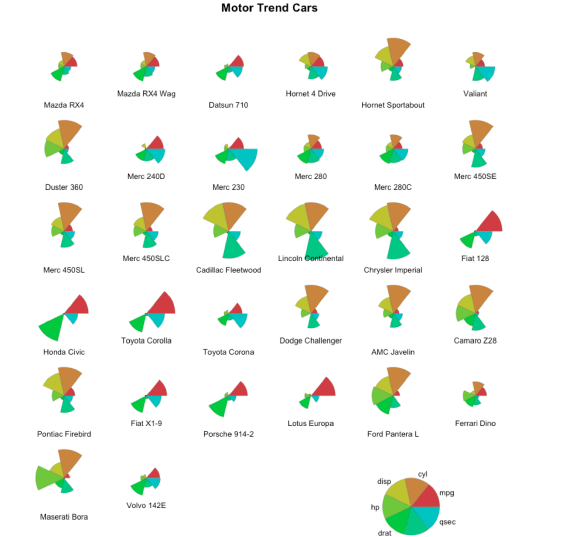
\includegraphics[width=.5\linewidth]{starplot}
\end{figure}
\end{itemize}

\subsubsection{Dimensionality reduction}
\begin{itemize}
\item \textbf{PCA}\\
Applied to reduce the number of dimensions of data (\textbf{feature selection}). The goal of PCA is to find a projection that captures the \textbf{largest amount of variation} in data. Given N data vectors from n-dimensions find k<n orthogonal vectors ( principal components) that can be used to represent data. Works for numerical data if \textbf{affected by scale}
\begin{enumerate}
\item Normalize data
\item Compute k orthonormal unit vectors (\textbf{principal components})
\item Each input vector is a \textbf{linear combination }of the k principal component vectors
\item The PC are sorted in order of \textbf{decreasing significance}
\end{enumerate}
\item \textbf{t-Distributed Stochastic Neighbour Embedding}\\
It is a \textbf{non-linear} dimensionality reduction technique used to map high dimensionality data to \textbf{two or three dimensions}. The algorithm converts \textbf{similarities} between data points to \textbf{joint probabilities} and model  high dimensional points into map points so that position of the map points aims at	conserving the structure of the data  (similar points are near, dissimilar points are far away)
\begin{enumerate}
\item Define a probability distribution over pairs of high dimensional data points so that \textbf{similar points} have high probability of being picked and \textbf{dissimilar points} have extremely small probability of being picked
\item Define a similar distribution over the points of the map space by minimizing (\textbf{gradient descent}) the distance of the \textbf{Kullback-Leibler} divergence between that two distributions with respect to the locations of the map points.
\end{enumerate}
Different initialisation will lead to different results and should be applied to data with a reasonable number of dimensions ( 30-50). With more dimensions other algorithms should be applied.
\end{itemize}

\subsubsection{Other visualisation techniques}
\begin{itemize}
\item \textbf{Contour plots}\\
Useful for continuous attributes measured on a spatial grid. They partition the plane into regions of similar values. The contour lines that form the boundaries of these regions connect points with equal values.
\item \textbf{Heat maps}\\
\begin{figure}[H]
 \centering
 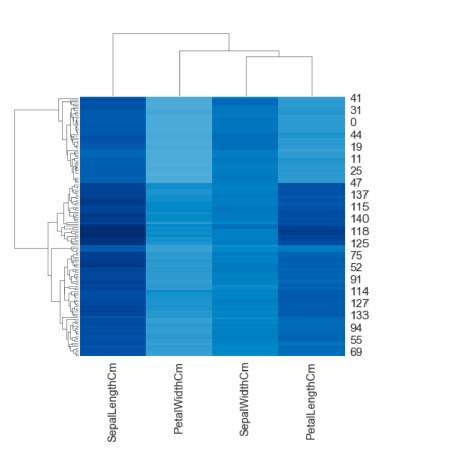
\includegraphics[width=.6\linewidth]{heatmaps}
\end{figure}
\end{itemize}